\begin{frame}
  \frametitle{Gastos del GNC \\ \small{Fuente: MHCP - CARF}}
  \begin{center}
    \resizebox{\textwidth}{!}{
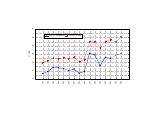
\begin{tikzpicture}[scale=0.08]
\begin{axis}[
    width=16.5cm,
    height=9.5cm,
    ylabel={\% PIB},
    % --- Ticks manuales para incluir 2025 y 2026 ---
    xtick={7,8,...,22},
    xticklabels={2011,2012,2013,2014,2015,2016,2017,2018,2019,2020,2021,2022,2023,2024,2025,2026},
    x tick label style={rotate=90, anchor=east},
    ymin=14,
    ymax=26,
    grid=both,
    grid style=dashed,
    minor y tick num=1,
    legend style={at={(0.3,0.9)}, anchor=north, legend columns=-1},
    thick
]

% Gasto Primario (histórico)
\addplot[
    color=blue,
    mark=*,
    very thick
] coordinates {
    (7,15.3) (8,15.8) 
    (9,16.8) (10,16.7) (11,16.5) (12,16.0) (13,16.4) (14,15.4) (15,15.8) (16,20.2) 
    (17,19.8) (18,17.2) (19,19.2) (20,19.0)
};

% Gasto Total (histórico)
\addplot[
    color=red,
    mark=square*,
    dashed
] coordinates {
    (7,18.0) (8,18.4) 
    (9,19.1) (10,18.9) (11,19.1) (12,18.9) (13,19.3) (14,18.2) (15,18.7) (16,23.1) 
    (17,23.1) (18,21.5) (19,23.1) (20,23.4)
};

% Proyecciones Gasto Primario (línea punteada)
\addplot[
    color=blue!60!black,
    dashed
] coordinates {
    (20,19.0) (21,19.7) (22,20.1)
};

% Proyecciones Gasto Total (línea punteada)
\addplot[
    color=red!60!black,
    dashed
] coordinates {
    (20,23.4) (21,22.9) (22,24.2)
};

% Puntos grises Gasto Primario
\addplot[
    color=gray,
    mark=*,
    only marks
] coordinates {
    (21,19.7) (22,20.1)
};

% Puntos grises Gasto Total
\addplot[
    color=gray,
    mark=square*,
    only marks
] coordinates {
    (21,22.9) (22,24.2)
};

\legend{Gasto Primario, Gasto Total}
\end{axis}
\end{tikzpicture}
}
  \end{center}
\end{frame}
